\chapter{Results}
In this chapter the experimental results will be presented. This will include the data analysis of both the magnetic field strength calibration, the hall coefficient and charge carrier density. The uncertainty calculations are also given.

\section{Magnetic field strength calibration}
The calibration result of the coils are visible in Figure \ref{fig:call_result}. It can be seen that the magnetic field strength created by the coils as a function of the current through them is
    \begin{equation}
        B(I) = 40,4 \cdot I + 0,7678 \label{eq:call}
    \end{equation}
with a correlation coefficient R$^2$ of 0,9995 and root-mean-square error (RMSE) of 1,35.

\section{Data analysis}
All data analysis has been done in Python. The code can be found in Appendix B. The correlation coefficient $R^2$ and standard error of the estimated gradient (stderr) are values given by the fit which is created with SciPy. The magnetic field strength calibration has been fitted by using MATLAB. 

\section{Results}
The results of sample 1-6 of the Hall voltage measurement of silver are visible in Figure \ref{fig:silver1-6}. In which
    \begin{equation}
        \frac{U_H}{I} = \frac{1}{n \cdot e} \frac{B}{d} \tag{\ref{eq:Hall Voltage2}}
    \end{equation}
is determined to be equal to
    \begin{equation}
        \frac{U_H}{I} = (0.558 \pm 0.005) \quad \text{[VA$^{-1}$]}. \label{eq:result_silver}
    \end{equation}
    \begin{figure}[!htbp]
    \begin{center}
    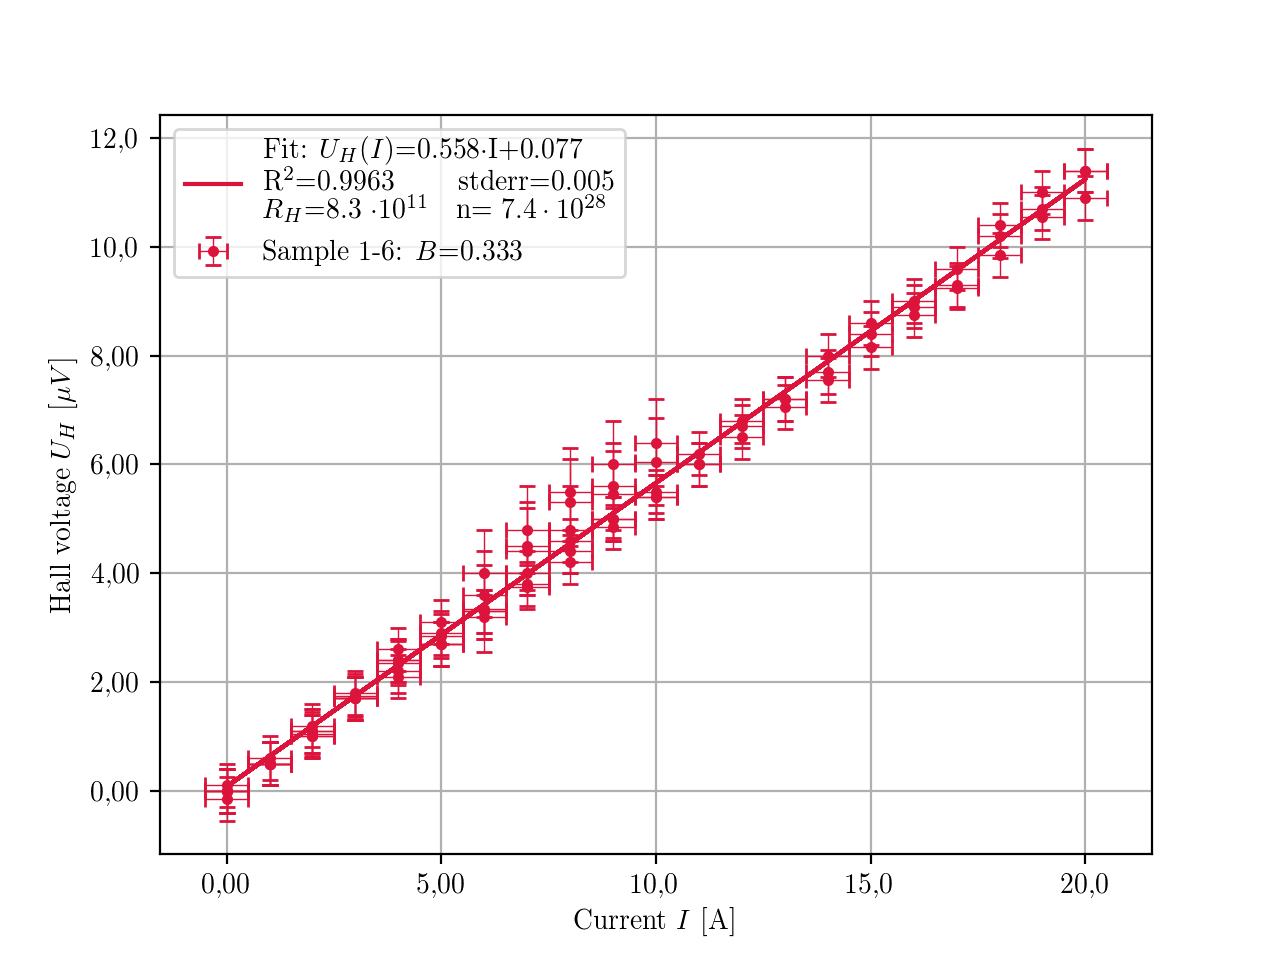
\includegraphics[scale=0.9]{figuren/resultaten/sample1-6.png}
    \end{center}
    \caption{Results of sample 1-6 of the Hall voltage measurement with the Hall apparatus (silver).}\label{fig:silver1-6}
    \end{figure}
    \begin{figure}[!htbp]
    \begin{center}
    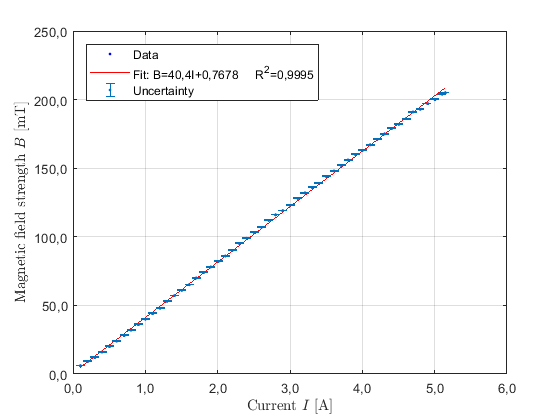
\includegraphics[scale=0.9]{figuren/resultaten/call_result.png}
    \end{center}
    \caption{Calibration of the magnetic field strength produced by the coils as a function of the current through the coils. This fit has a RMSE of 1,35.}\label{fig:call_result}
    \end{figure}
This gives a Hall coefficient of
    \begin{equation}
        R_H = \frac{U_H}{I} \frac{d}{B}
    \end{equation}
    
    \begin{equation}
        R_H = 0.558 \cdot 10^{-6} \cdot \frac{5\cdot 10^{-5}}{0.333} \quad \text{[m$^3$C$^{-1}$]}
    \end{equation}
    
    \begin{equation}
        R_H = (8.3 \pm 2) \cdot 10^{-11} \quad \text{[m$^3$C$^{-1}$]}
    \end{equation}
and a charge carrier density of
    \begin{equation}
        n = (7.4 \pm 2)\cdot 10^{28} \quad \text{[m$^{-3}$]}.
    \end{equation}
In which both the uncertainties are equal to the standard deviation of individual results from sample 1-6. These results can be found in Appendix A.

\section{Uncertainty calculations}
The hall coefficient $R_H$ is calculated as follows.
    \begin{equation}
        R_H = \frac{U_H}{I} \frac{d}{B} \label{eq:hallcoefficient}
    \end{equation}
Of which its uncertainty has to be determined. The uncertainty of $d$ is not known. Therefor it is estimated to be in the same order of magnitude as its given value. Silver for example with a plate thickness $d$ = 5 \cdot 10$^{-5}$ m \cite{apparatus_silver}, will have an estimated uncertainty of:
    \begin{equation}
        \Delta d = 1\cdot 10^{-5} \quad \text{[m]}
    \end{equation}
For $\Delta B$ the RMSE of the linear regression fit will be used. For $\Delta \frac{U_H}{I}$ the standard error of the estimated gradient (STDERR) will be used. These are calculated respectively by MATLAB and SciPy, see Appendix B for more information. Finally $\Delta R_H$ has to be determined. This is done by using propagation of uncertainty \cite{error_propagation}:
    \begin{equation}
        s_f = \sqrt{\bigg(\frac{\partial f}{\partial x}\bigg)^2 s_x^2 +
        \bigg(\frac{\partial f}{\partial y}\bigg)^2 s_y^2 +
        \bigg(\frac{\partial f}{\partial z}\bigg)^2 s_z^2 + ...} \label{eq:errorpropagation}
    \end{equation}
where $s_f$ represents the standard deviation of the function $f$. The standard deviation of x, y, z is represented by respectively $s_x$, $s_y$, $s_z$. Writing Equation \ref{eq:hallcoefficient} in the form of Equation \ref{eq:errorpropagation} results in:
\begin{equation}
    \Delta R_H = \sqrt{
    \bigg(\frac{d}{B}\bigg)^2 \cdot \bigg(\Delta \frac{U_H}{I}\bigg)^2 +
    \bigg( \frac{U_H}{I} \frac{1}{B} \bigg)^2 \cdot \bigg( \Delta d \bigg)^2 +
    \bigg( - \frac{U_H}{I} \frac{d}{B^2}\bigg)^2 \cdot \bigg( \Delta B \bigg)^2
    }
\end{equation}
In which $\frac{U_H}{I}$ is assumed to be one variable, since its uncertainty is equal to the STDERR given by the fit of $\frac{U_H}{I}$ done in Python.
The error $\Delta x$ in the final result of the Hall coefficient $R_H$ and charge carrier density $n$ is calculated by using the standard error of the mean which is given by \cite{researchmethods}:
    \begin{equation}
        \Delta x \approx \frac{s}{\sqrt{N}}
    \end{equation}
In which $s$ equals the standard deviation in the data set and $N$ equals the number of samples.

    \begin{figure}[!htbp]
    \begin{center}
    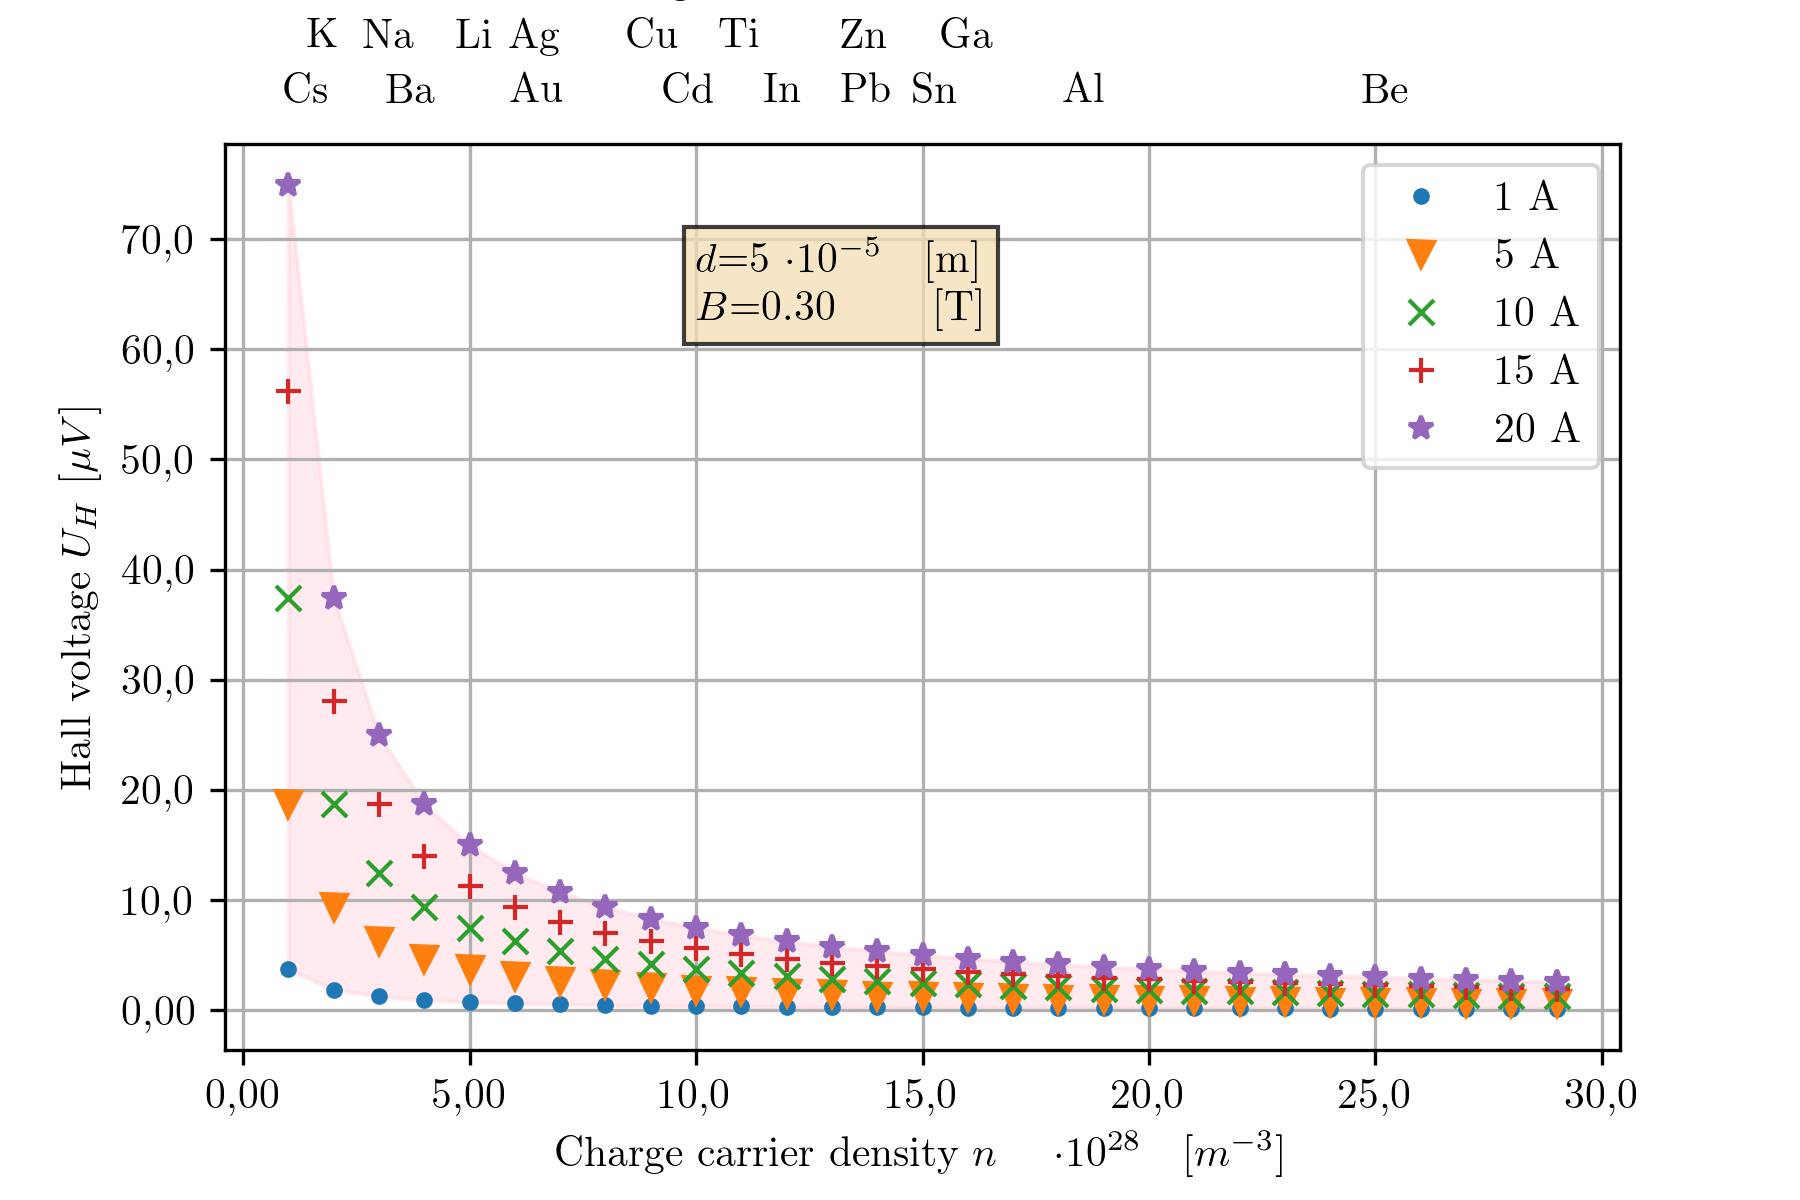
\includegraphics[scale=0.85]{figuren/simulatie/n.png}
    \end{center}
    \caption{Simulation result of Equation \ref{eq:Hall Voltage2}, with above of the figure the charge carrier densities ofdifferent materials \cite{ccdensity}.} \label{fig:sim_n}
    \end{figure}

\section{Python simulation}
Figure \ref{fig:sim_n} shows the Hall voltage for different materials with a different charge carrier density. It can be seen that silver (Ag) for example, with a charge carrier density  of $n \approx 6,5\cdot 10^{28}$ m$^{-3}$, has a Hall voltage of $U_H \approx 11 \mu$V in a magnetic field of 0,3 T with a plate width of $5 \cdot 10^{-5}$ m. It is also visible that cesium (Cs) and kalium (K) have a higher Hall voltage than silver (Ag). In others words, their Hall coefficient is higher. \\
More simulations results can be found in Appendix A. In Figure \ref{fig:sim_B} all variables except the magnetic field strength $B$ have been kept constant. The same goes for Figure \ref{fig:sim_I}, but in this case the current $I$ is the changing variable. Both of these figures can be used to verify experimental results while measuring. Figure \ref{fig:sim_d} shows that a change in conductor thickness $d$ in the magnitude of 10$^{-5}$ does not have any significant impact on the Hall voltage. This is as excepted, since the conductor thickness is multiple orders of magnitude smaller than the generated Hall voltage in this physical situation. The Python code used to create these figures can be found in Appendix B.